\documentclass[xetex,mathserif,serif]{beamer}
\usepackage{polyglossia}
\setdefaultlanguage[babelshorthands=true]{russian}
\usepackage{minted}
\usepackage{tabu}
\usepackage{pgfplots}
\usepackage{textpos}
\usepackage{subcaption}
\usepackage{graphicx}
\usepackage[normalem]{ulem}
\usepackage{algorithm2e}
\usepackage{algorithmic}
\usepackage{float}
\useoutertheme{infolines}

\usepackage{fontspec}
\setmainfont{FreeSans}
\newfontfamily{\russianfonttt}{FreeSans}

\usepackage{forest}
\usetikzlibrary{arrows}

\definecolor{links}{HTML}{2A1B81}
\hypersetup{colorlinks,linkcolor=,urlcolor=links}

\newcommand{\attribution}[1] {
    \vspace{-5mm}\begin{flushright}\begin{scriptsize}\textcolor{gray}{\textcopyright\, #1}\end{scriptsize}\end{flushright}
}

\tabulinesep=0.7mm

\title{Обзор парадигм программирования}
\subtitle{Часть 2}
\author[Юрий Литвинов]{Юрий Литвинов \newline \textcolor{gray}{\small\texttt{y.litvinov@spbu.ru}}}

\date{30.11.2021}

\begin{document}
    
    \frame{\titlepage}

    \begin{frame}
        \frametitle{Логическое программирование}
        \begin{itemize}
            \item Программа представляет собой набор фактов и правил, система сама строит решение с использованием правил логики
            \begin{itemize}
                \item Использует логику предикатов как математическую формализацию
            \end{itemize}
            \item Создавалось в 60-х для решения задач искусственного интеллекта и экспертных систем
            \begin{itemize}
                \item Автоматическое доказательство теорем
            \end{itemize}
            \item Могут использоваться разные стратегии доказательства
            \begin{itemize}
                \item В общем случае, программа --- это набор фактов и правил + стратегия вывода, которая управляет тем, как новые факты получаются из существующих
                \begin{itemize}
                    \item В формальной логике стратегия вывода обычно не важна, для компьютеров это критично
                \end{itemize}
            \end{itemize}
            \item Дедуктивные базы данных --- хранят факты и правила вывода
        \end{itemize}
    \end{frame}

    \begin{frame}
        \frametitle{Пролог}
        \begin{itemize}
            \item Появился в 1972 г. как научная разработка
            \item Реализации:
            \begin{itemize}
                \item SWI-Prolog (\url{http://www.swi-prolog.org/})
                \item Amzi Prolog (\url{http://www.amzi.com/})
                \item Turbo Prolog
            \end{itemize}
            \item Использует метод резолюций – последовательно перебирая правила и факты, пытается подобрать такой набор переменных, которые бы им удовлетворяли
            \begin{itemize}
                \item Пример:
                \begin{itemize}
                    \item cat(tom)
                    \item ?- cat(tom).

                        Yes
                    \item ?- cat(X).

                        X = tom
                \end{itemize}
            \end{itemize}
        \end{itemize}
    \end{frame}

    \begin{frame}[fragile]
        \frametitle{Пример программы}
        \begin{minted}{prolog}
sibling(X, Y) :- parent_child(Z, X), parent_child(Z, Y).
parent_child(X, Y) :- father_child(X, Y).
parent_child(X, Y) :- mother_child(X, Y).
mother_child(trude, sally).
father_child(tom, sally).
father_child(tom, erica).
father_child(mike, tom).

?- sibling(sally, erica).
Yes
?- father_child(Father, Child).
        \end{minted}
    \end{frame}

    \begin{frame}[fragile]
        \frametitle{Императивное программирование}
        \begin{minted}{prolog}
?- write('Hello world!'), nl.
Hello world!
true.

program_optimized(Prog0, Prog) :-
    optimization_pass_1(Prog0, Prog1),
    optimization_pass_2(Prog1, Prog2),
    optimization_pass_3(Prog2, Prog).
        \end{minted}
    \end{frame}

    \begin{frame}[fragile]
        \frametitle{QSort}
        \begin{minted}{prolog}
quicksort(Xs, Ys) :- quicksort_1(Xs, Ys, []).

quicksort_1([], Ys, Ys).
quicksort_1([X|Xs], Ys, Zs) :-
    partition(Xs, X, Ms, Ns),
    quicksort_1(Ns, Ws, Zs),
    quicksort_1(Ms, Ys, [X|Ws]).
 
partition([K|L], X, M, [K|N]):-
    X < K, !,
    partition(L, X, M, N).
partition([K|L], X, [K|M], N):-
    partition(L, X, M, N).
partition([], _, [], []).
        \end{minted}
    \end{frame}

    \begin{frame}
        \frametitle{Рекурсивное программирование, РЕФАЛ}
        \begin{itemize}
            \item РЕкурсивных Функций АЛгоритмический
            \begin{itemize}
                \item В. Турчин, 1966г.
            \end{itemize}
            \item Ориентирован на символьные вычисления
            \begin{itemize}
                \item ИИ, перевод, манипуляции с формальными системами (лямбда-исчисление, например)
            \end{itemize}
            \item Использует нормальные алгорифмы Маркова в качестве математической формализации
            \item Программа записывается в виде набора функций
            \begin{itemize}
                \item Функция --- упорядоченный набор предложений
                \item Предложение состоит из шаблона и того, на что надо заменить шаблон
                \item Выражения в угловых скобках (активные выражения)
                \item Переменные
            \end{itemize}
            \item Вычисление продолжается, пока в <<поле зрения>> Рефал-машины не окажется выражение без угловых скобок
        \end{itemize}
    \end{frame}

    \begin{frame}[fragile]
        \frametitle{Рефал, пример}
        Hello, world:
        \begin{minted}{text}
$ENTRY Go { = <Hello>;}
Hello {
   = <Prout 'Hello world'>;
}
        \end{minted}
        \vspace{3mm}
        Палиндром:
        \begin{minted}{text}
Palindrom {
    s.1 e.2 s.1 = <Palindrom e.2> ;
    s.1 = True ;
    = True;
    e.1 = False ;
}
        \end{minted}
    \end{frame}
    
    \begin{frame}
        \frametitle{Переписывание графов}
        \framesubtitle{EMF Refactor}
        \begin{center}
            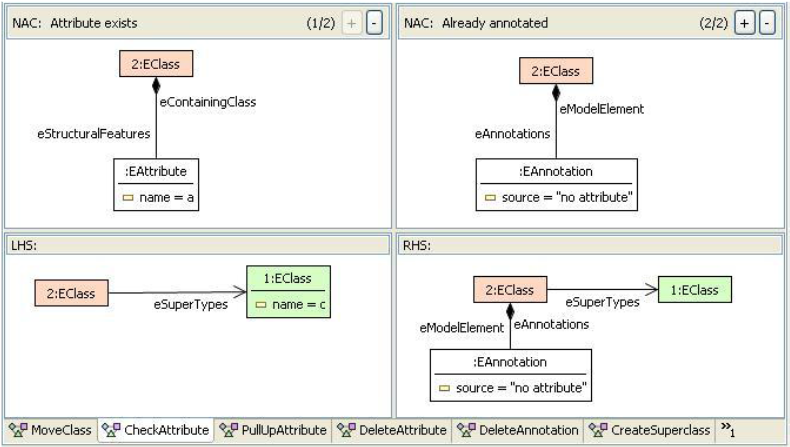
\includegraphics[width=0.8\textwidth]{graphRewriting.png}
        \end{center}
    \end{frame}

    \begin{frame}
        \frametitle{Стековое программирование}
        \begin{itemize}
            \item Язык Форт (Forth)
            \begin{itemize}
                \item Разработан в 60-х Чарльзом Муром <<для себя>>
                \item Был широко распространён для программирования встроенных систем и задач, естественным образом выражающихся в терминах стеков
                \begin{itemize}
                    \item Синтаксический анализ
                    \item Анализ естественных языков
                \end{itemize}
            \end{itemize}
        \end{itemize}
    \end{frame}

    \begin{frame}
        \frametitle{Форт, подробнее}
        \begin{itemize}
            \item Основной элемент программы: слово
            \item Форт-система состоит из словаря (набора слов) и стеков --- арифметического и командного (с их помощью производятся вычисления)
            \item Используется обратная польская нотация
        \end{itemize}
    \end{frame}

    \begin{frame}
        \frametitle{Примеры}
        \begin{columns}
            \begin{column}{0.82\textwidth}
                \begin{itemize}
                    \item \mintinline{forth}|25 10 * 50 + .|

                        Вывод: 300 ok
                    \item \mintinline{forth}|: FLOOR5 ( n -- n' )   DUP 6 < IF DROP 5 ELSE 1 -| \\
                        \mintinline{forth}|  THEN ;|
                    \begin{itemize}
                        \item то же самое на C:

                        \mintinline{c}|int floor5(int v) { return v < 6 ? 5 : v - 1; }|
                    \end{itemize}
                    \item более красиво на Форте:

                        \mintinline{forth}|: FLOOR5 ( n -- n' ) 1- 5 MAX ;|
                    \item \mintinline{forth}|: HELLO  ( -- )  CR ." Hello, world!" ;|
                \end{itemize}
            \end{column}
            \begin{column}{0.18\textwidth}
                \begin{center}
                    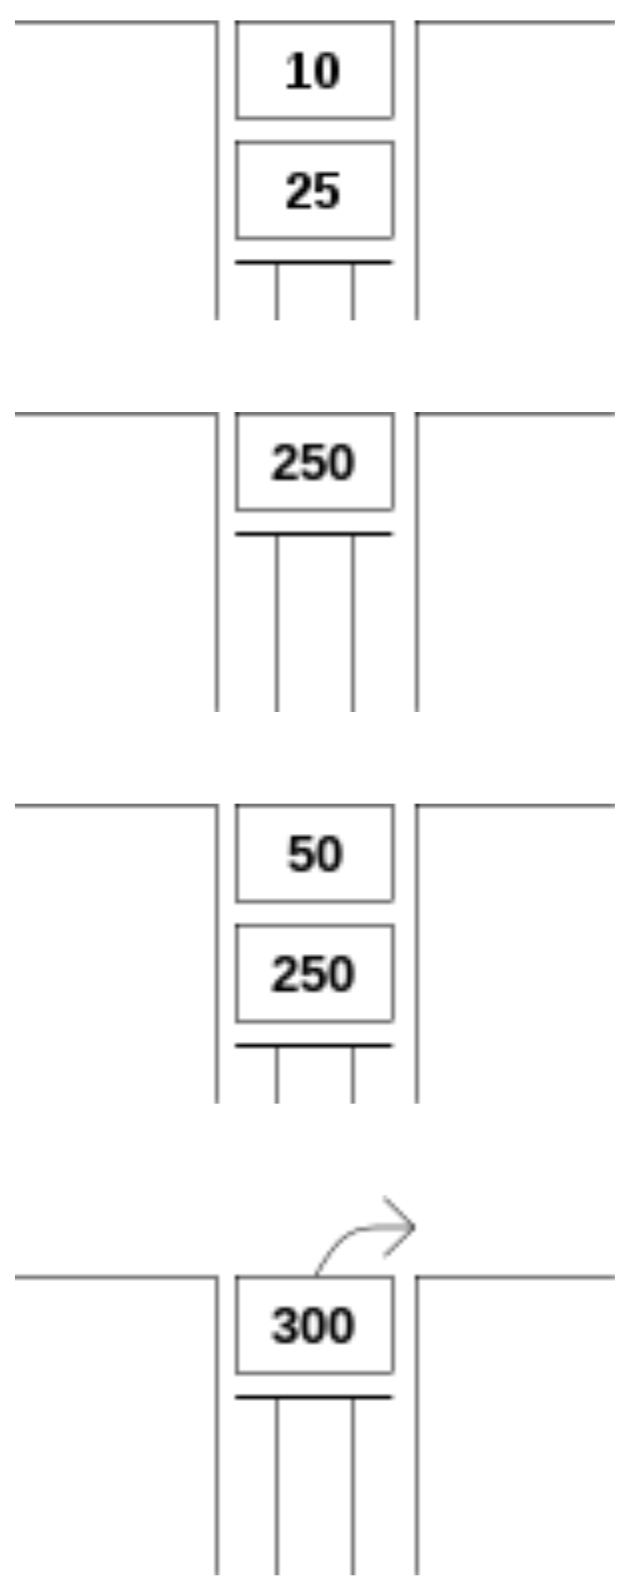
\includegraphics[width=\textwidth]{forthStack.png}
                \end{center}
            \end{column}
        \end{columns}
    \end{frame}

    \begin{frame}[fragile]
        \frametitle{Форт, пример}
        \begin{minted}{forth}
\ Напечатать знак числа
: .SIGN ( n -- )
   ?DUP 0= IF
     ." НОЛЬ"
   ELSE
     0> IF
     ." ПОЛОЖИТЕЛЬНОЕ ЧИСЛО" ELSE
     ." ОТРИЦАТЕЛЬНОЕ ЧИСЛО" THEN
   THEN
;
        \end{minted}
    \end{frame}

    \begin{frame}
        \frametitle{Реализации}
        \begin{columns}
            \begin{column}{0.8\textwidth}
                \begin{itemize}
                    \item SwiftForth
                    \begin{itemize}
                        \item \url{https://www.forth.com/swiftforth/}
                    \end{itemize}
                    \item Gforth
                    \begin{itemize}
                        \item \url{http://www.gnu.org/software/gforth/}
                    \end{itemize}
                    \item Десятки других реализаций
                    \begin{itemize}
                        \item \url{http://www.forth.org/commercial.html}
                    \end{itemize}
                    \item Книжка
                    \begin{itemize}
                        \item Броуди Л. <<Начальный курс программирования на Форте>>
                    \end{itemize}
                \end{itemize}
            \end{column}
            \begin{column}{0.2\textwidth}
                \begin{center}
                    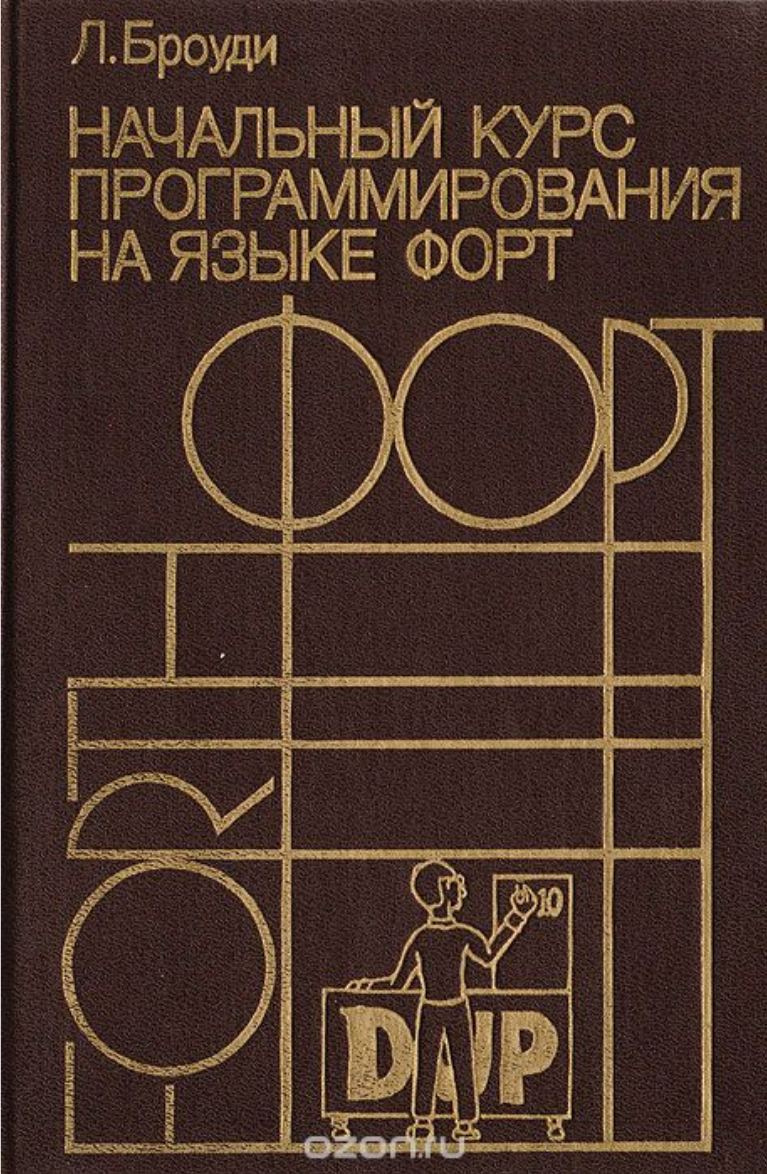
\includegraphics[width=\textwidth]{forthBookCover.png}
                \end{center}
            \end{column}
        \end{columns}
    \end{frame}

    \begin{frame}
        \frametitle{Визуальное программирование}
        \begin{itemize}
            \item Визуальные языки появились ещё до компьютеров
            \begin{itemize}
                \item Диаграммы потоков данных
                \item Сети Петри
            \end{itemize}
            \item Применяются прежде всего для моделирования, а не для программирования
            \begin{itemize}
                \item Описание архитектуры системы (UML, SysML, IDEFx)
                \item Описание бизнес-процессов (UML, BPMN)
                \item Описание схем баз данных (ER, ORM)
            \end{itemize}
            \item Есть и языки программирования: G (LabVIEW), Simulink, ДРАКОН, Scratch
            \item Предметно-ориентированные визуальные языки
            \begin{itemize}
                \item TRIK Studio
            \end{itemize}
        \end{itemize}
    \end{frame}

    \begin{frame}
        \frametitle{Пример (Matlab/Simulink)}
        \begin{center}
            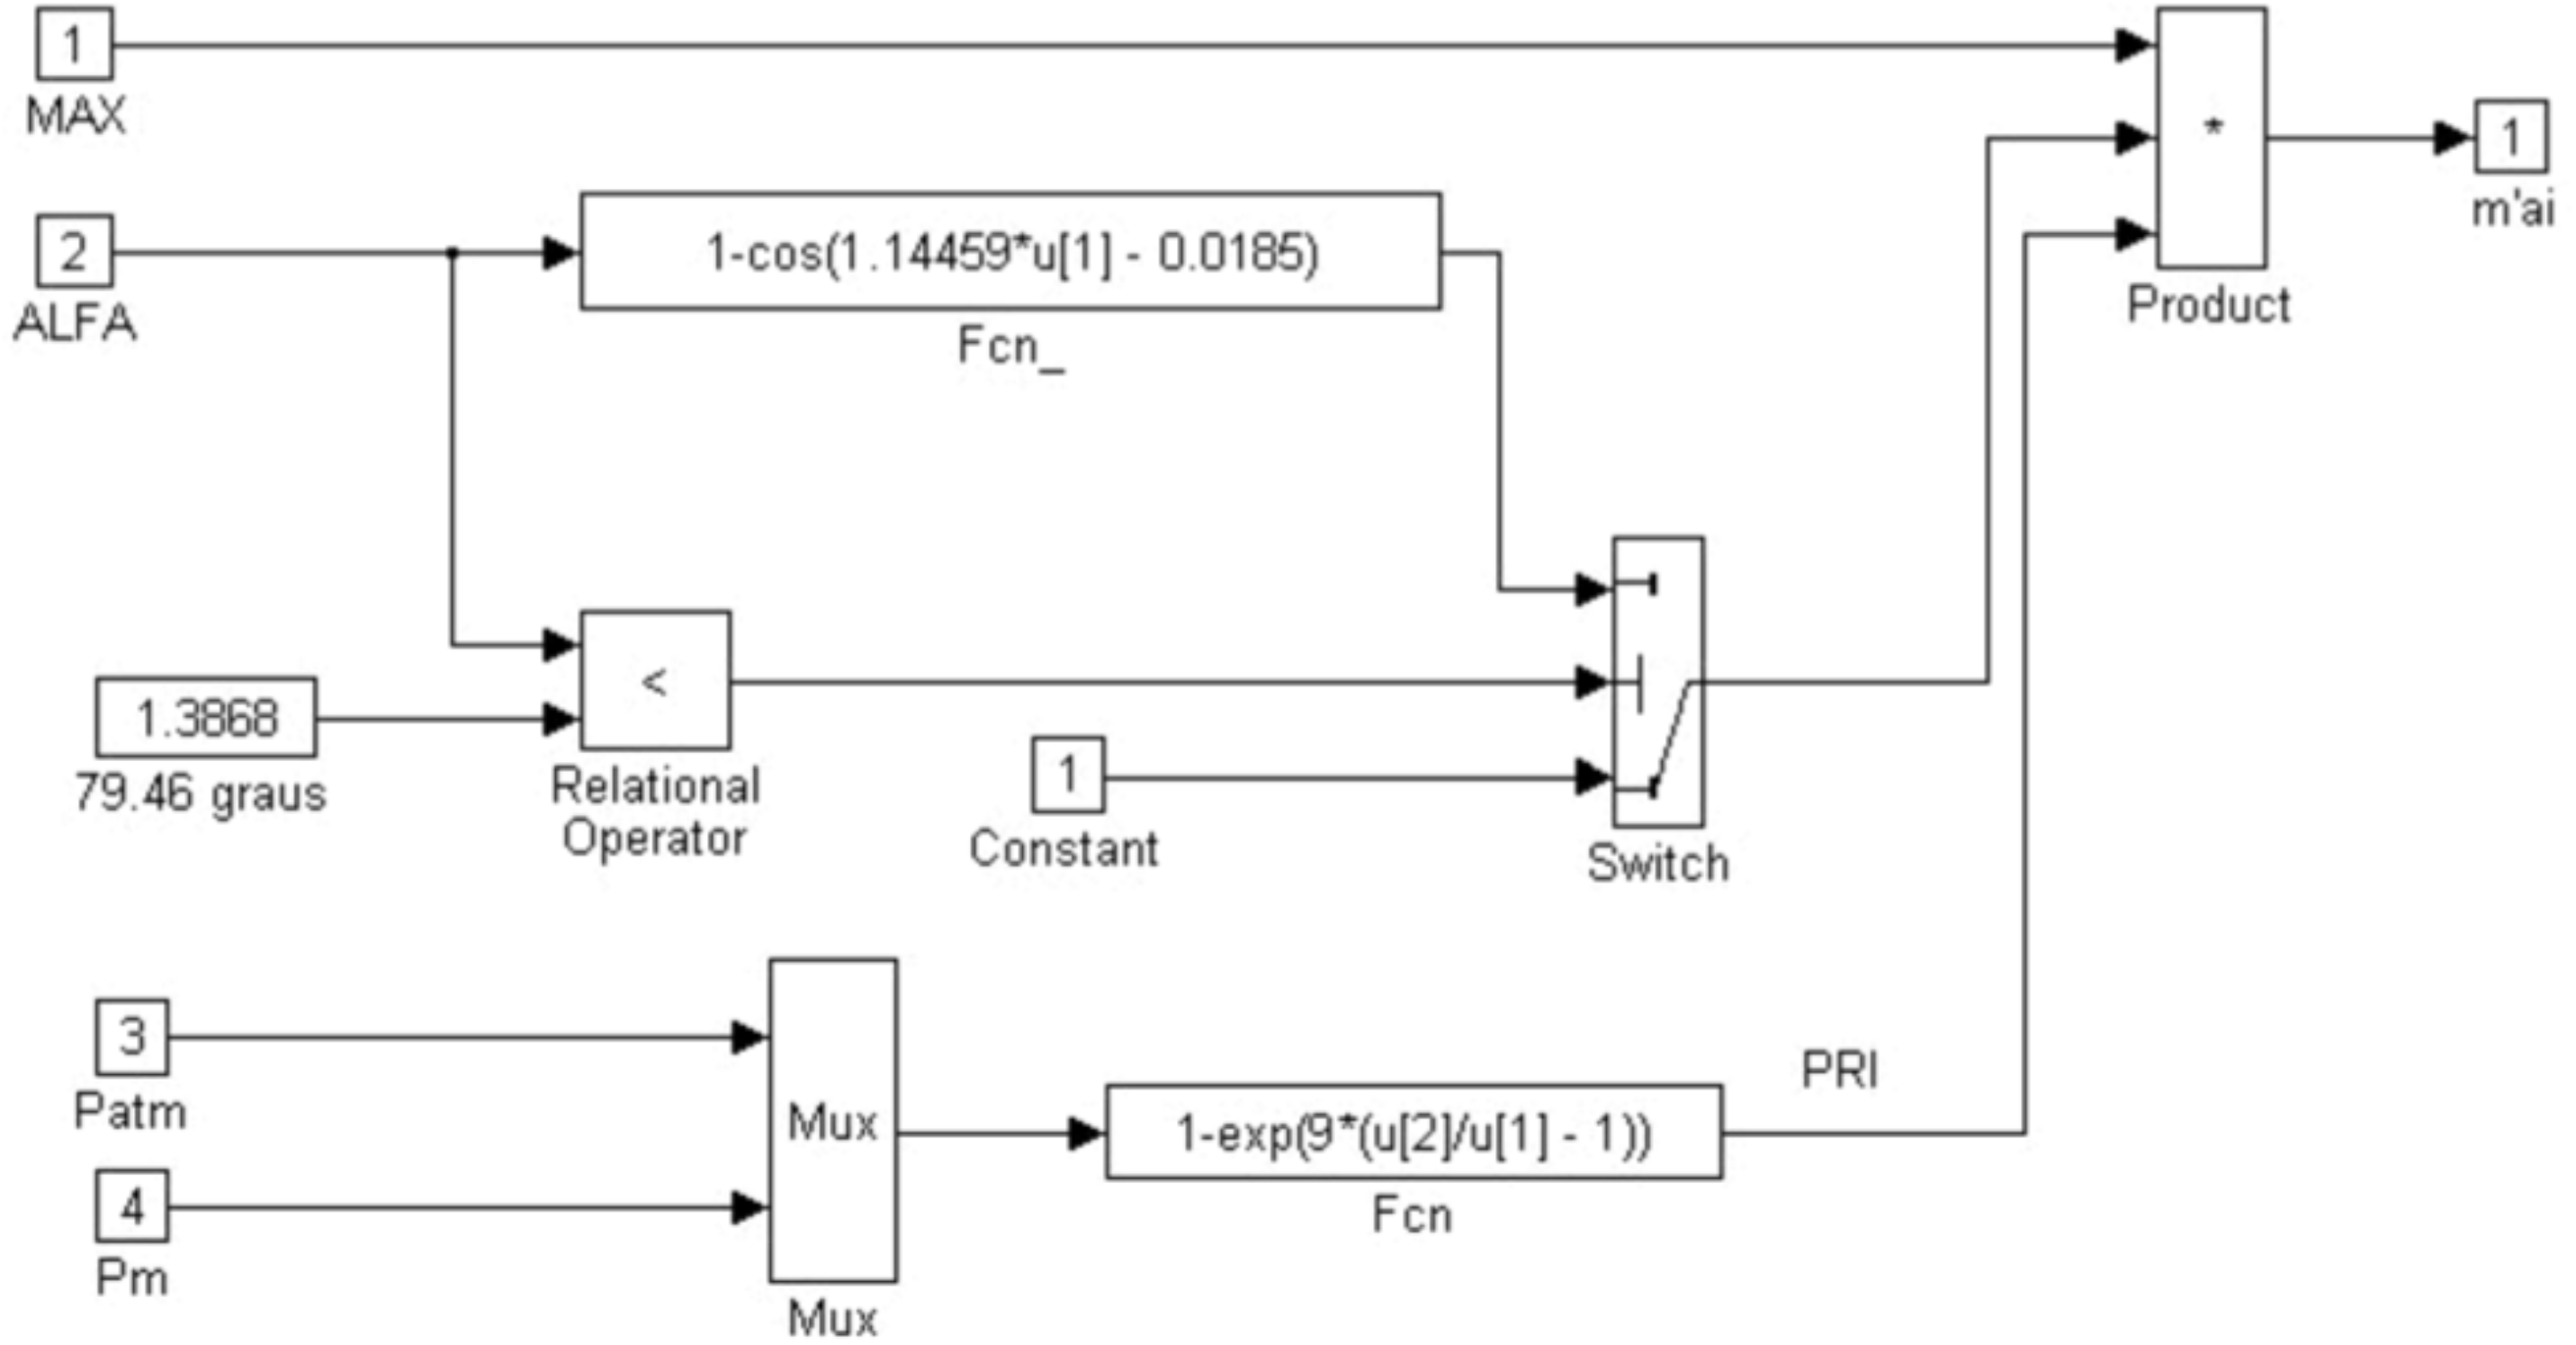
\includegraphics[width=0.9\textwidth]{simulink.png}
        \end{center}
    \end{frame}

    \begin{frame}
        \frametitle{Пример (LabVIEW)}
        \begin{center}
            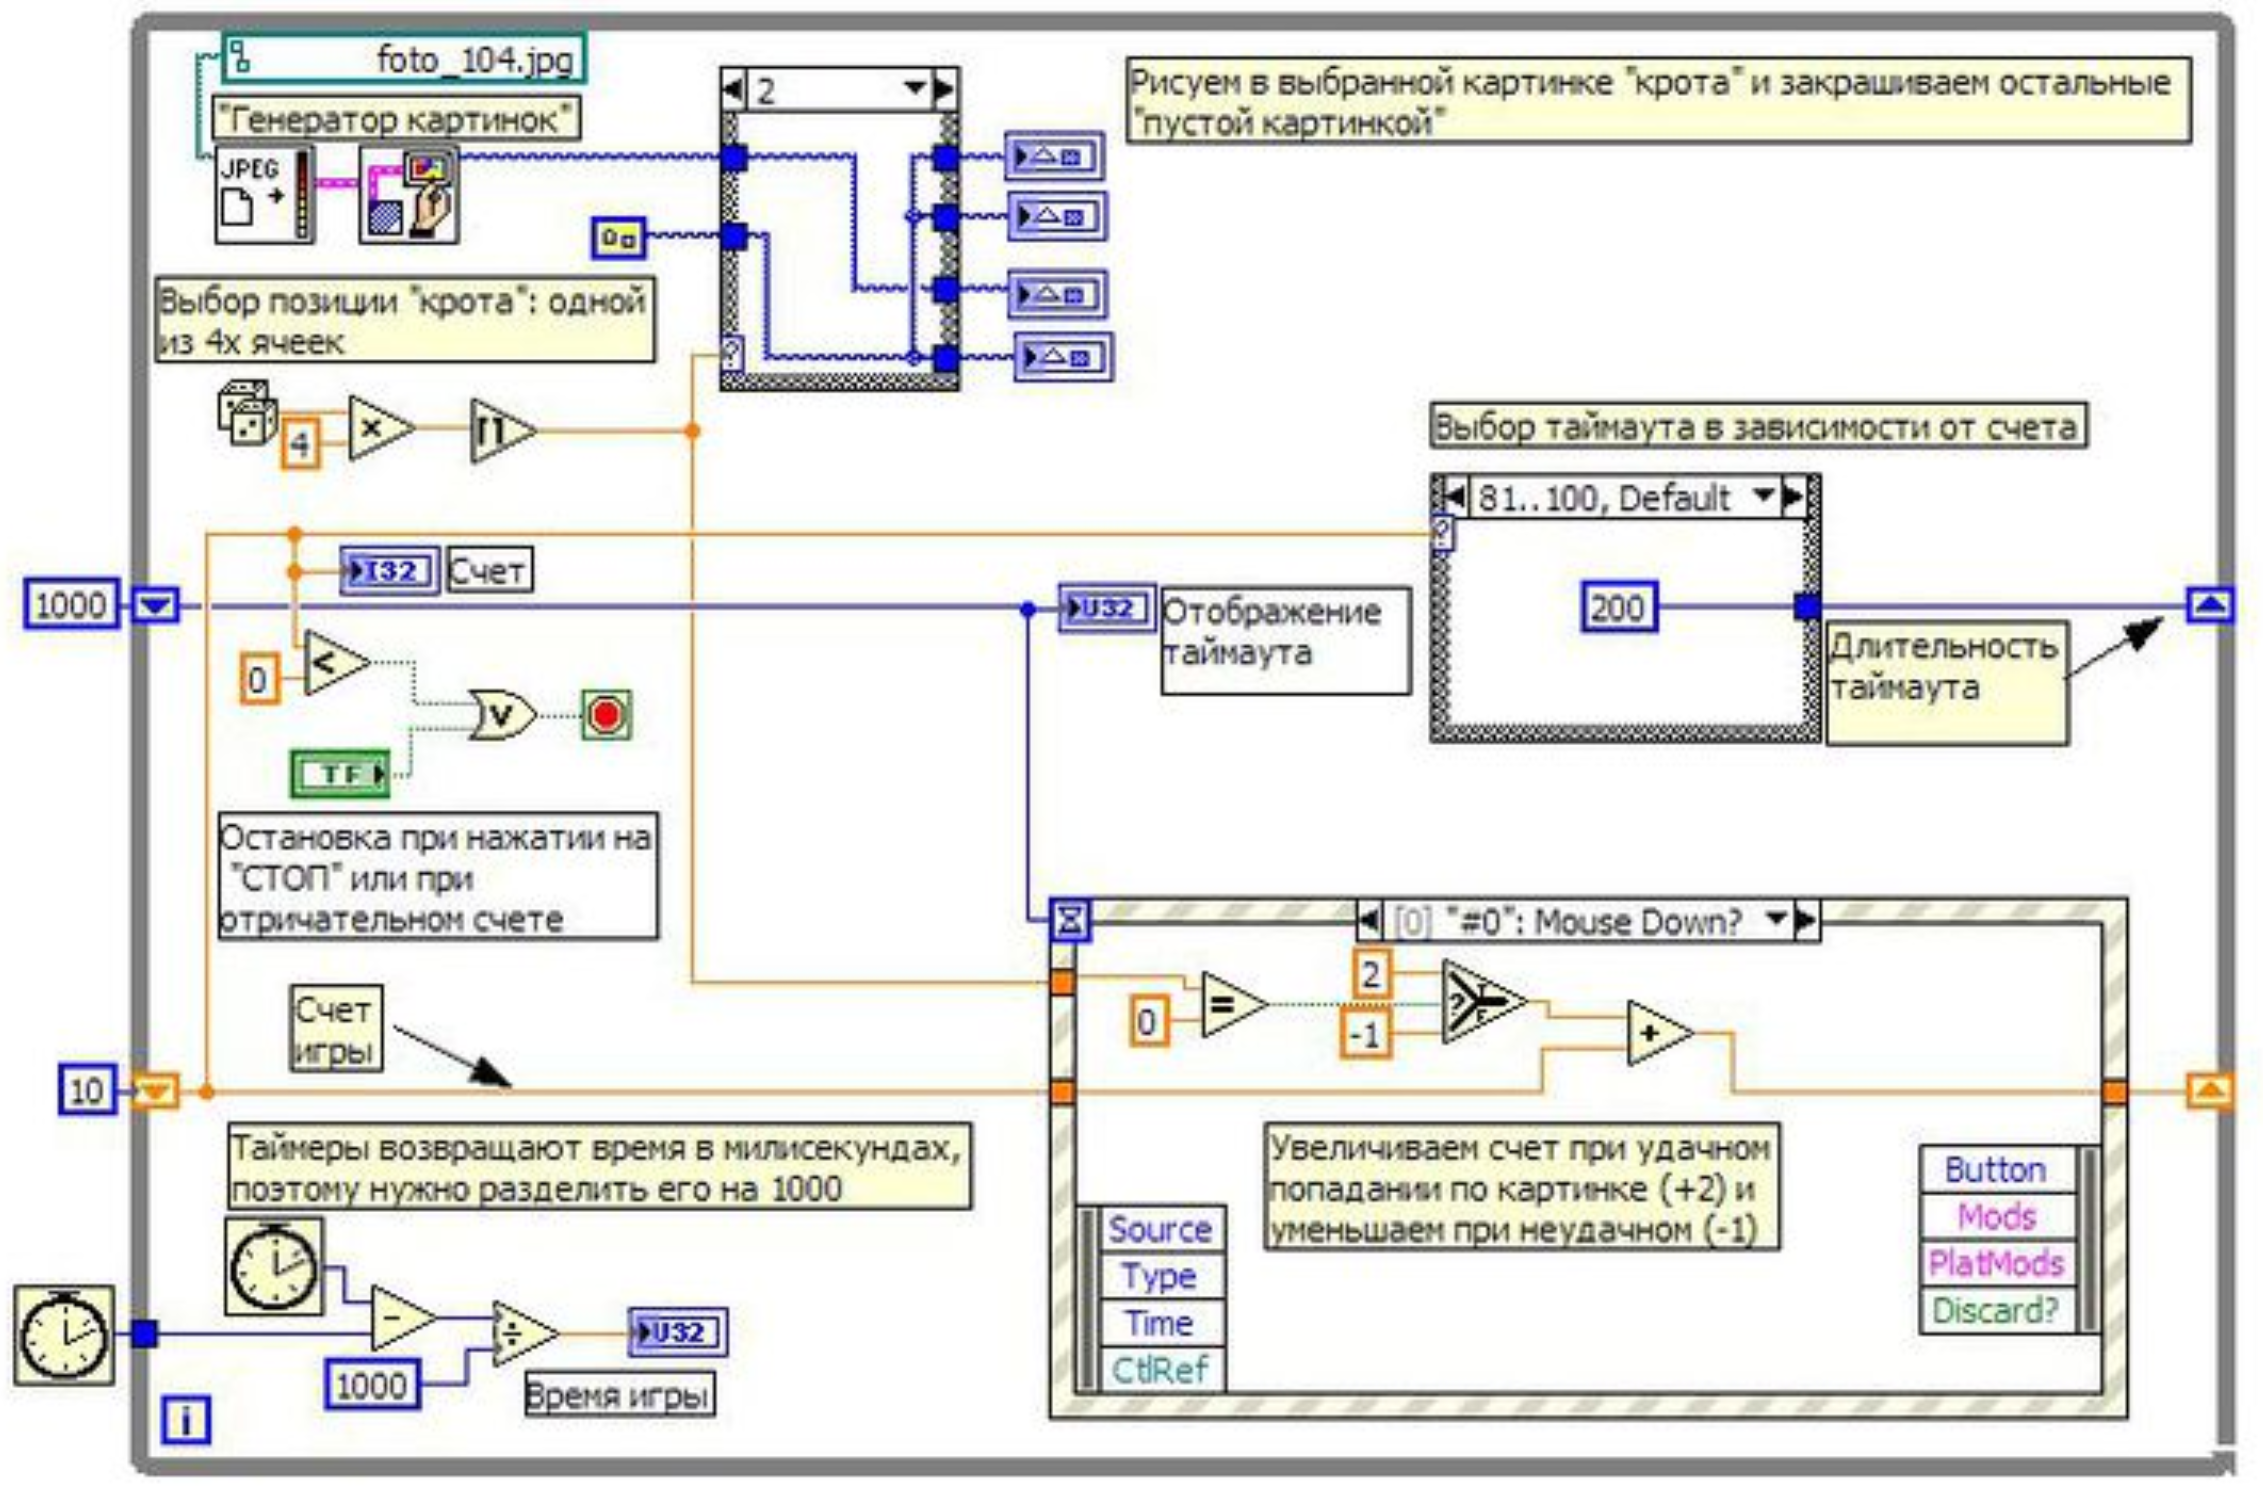
\includegraphics[width=0.8\textwidth]{labView.png}
        \end{center}
    \end{frame}

    \begin{frame}
        \frametitle{Пример (ДРАКОН)}
        \begin{center}
            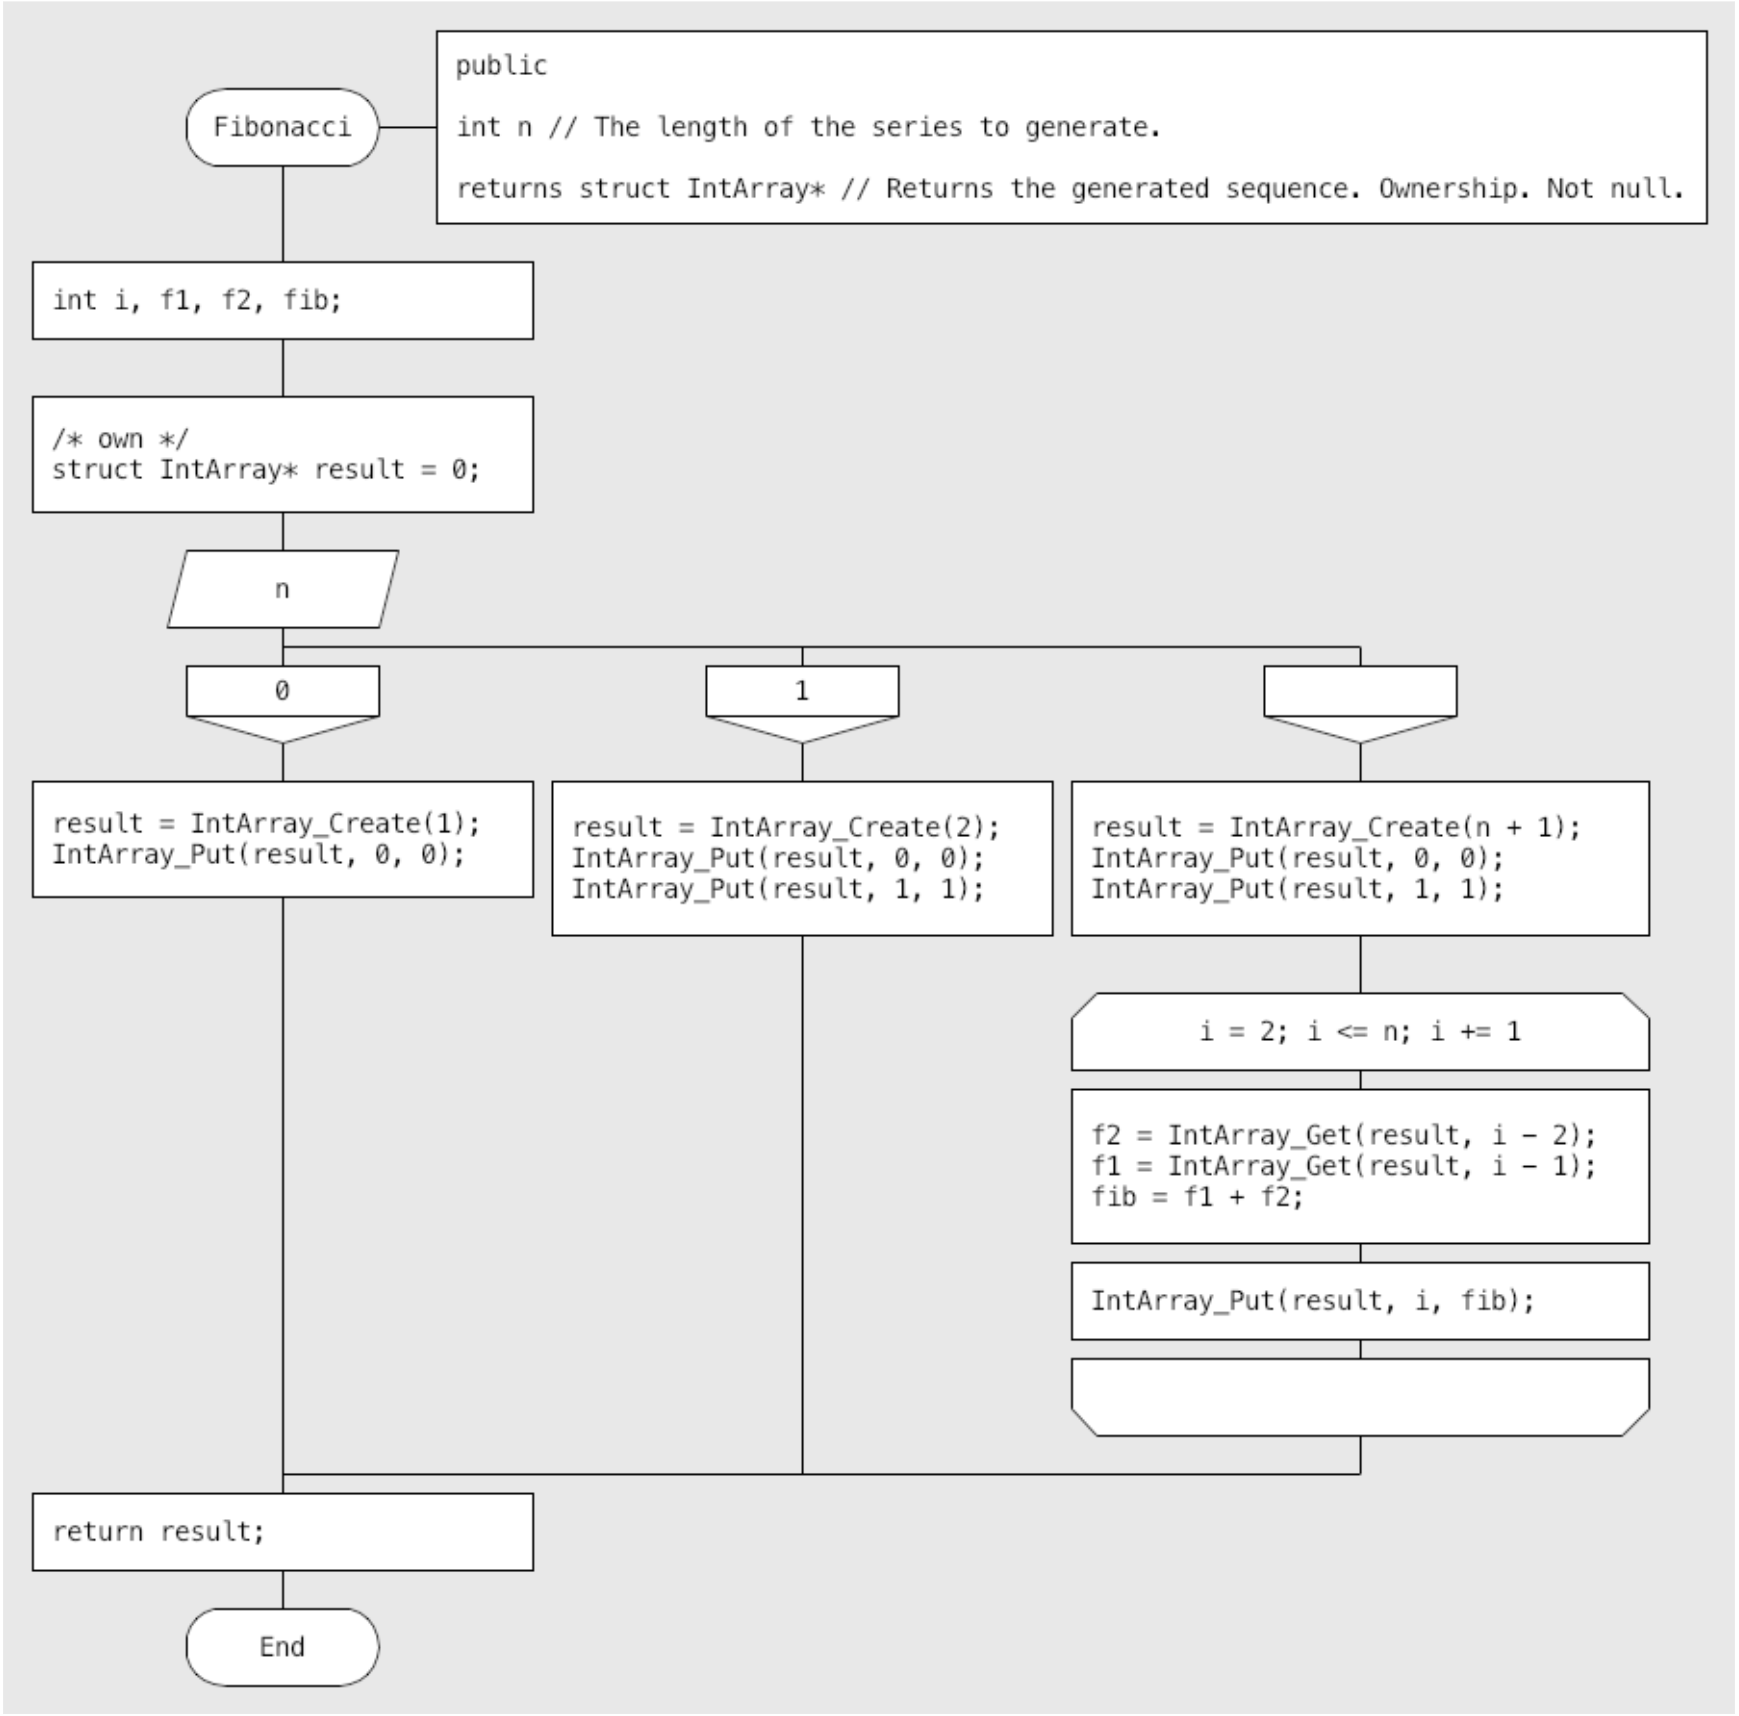
\includegraphics[width=0.6\textwidth]{drakon.png}
        \end{center}
    \end{frame}

    \begin{frame}
        \frametitle{Визуальное моделирование}
        \begin{columns}
            \begin{column}{0.7\textwidth}
                \begin{itemize}
                    \item Не ставит своей целью получить работающую программу
                    \item Модель проще, чем нужно исполнителю
                    \item Модель даже для сложной системы обозрима
                    \item Система описывается с разных дополняющих друг друга точек зрения
                    \begin{itemize}
                        \item При этом описание системы остаётся целостным, визуальная модель --- это не просто картинка
                    \end{itemize}
                    \item Модели можно анализировать до реализации
                    \item Могут быть сгенерированы заглушки классов и иногда даже реализации методов
                \end{itemize}
            \end{column}
            \begin{column}{0.3\textwidth}
                \begin{center}
                    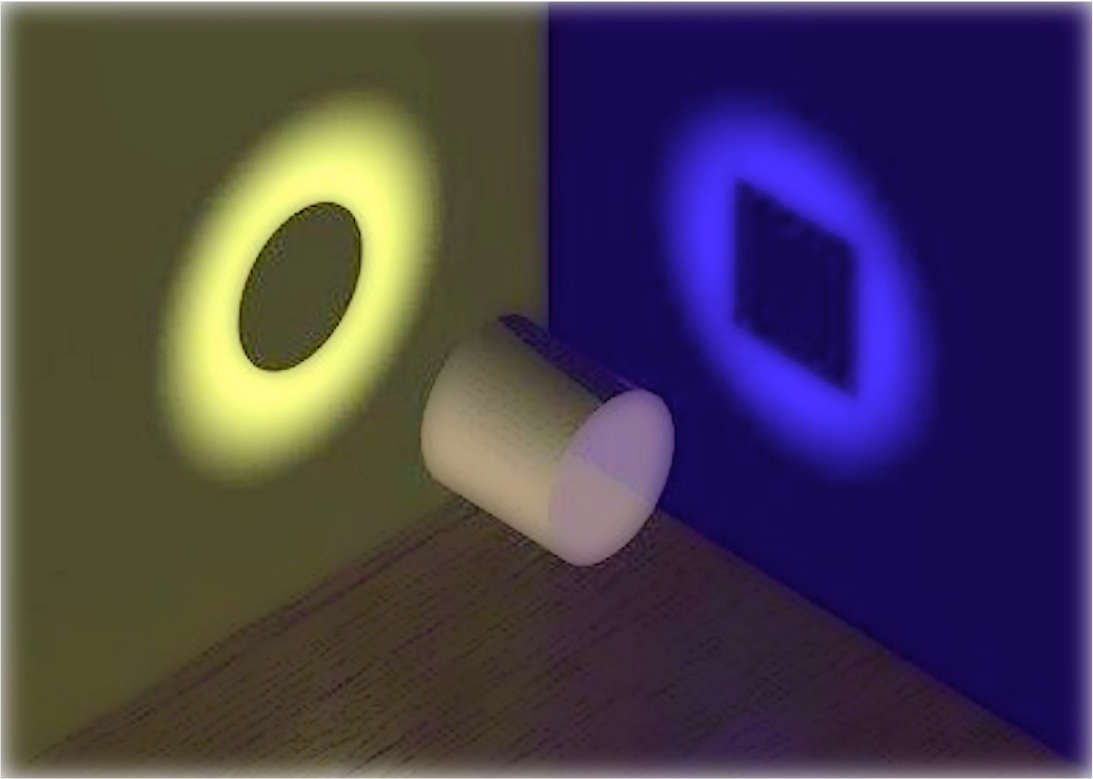
\includegraphics[width=\textwidth]{pointsOfView.png}
                \end{center}
            \end{column}
        \end{columns}
    \end{frame}

    \begin{frame}
        \frametitle{Пример высокоуровневой модели (UML)}
        \begin{center}
            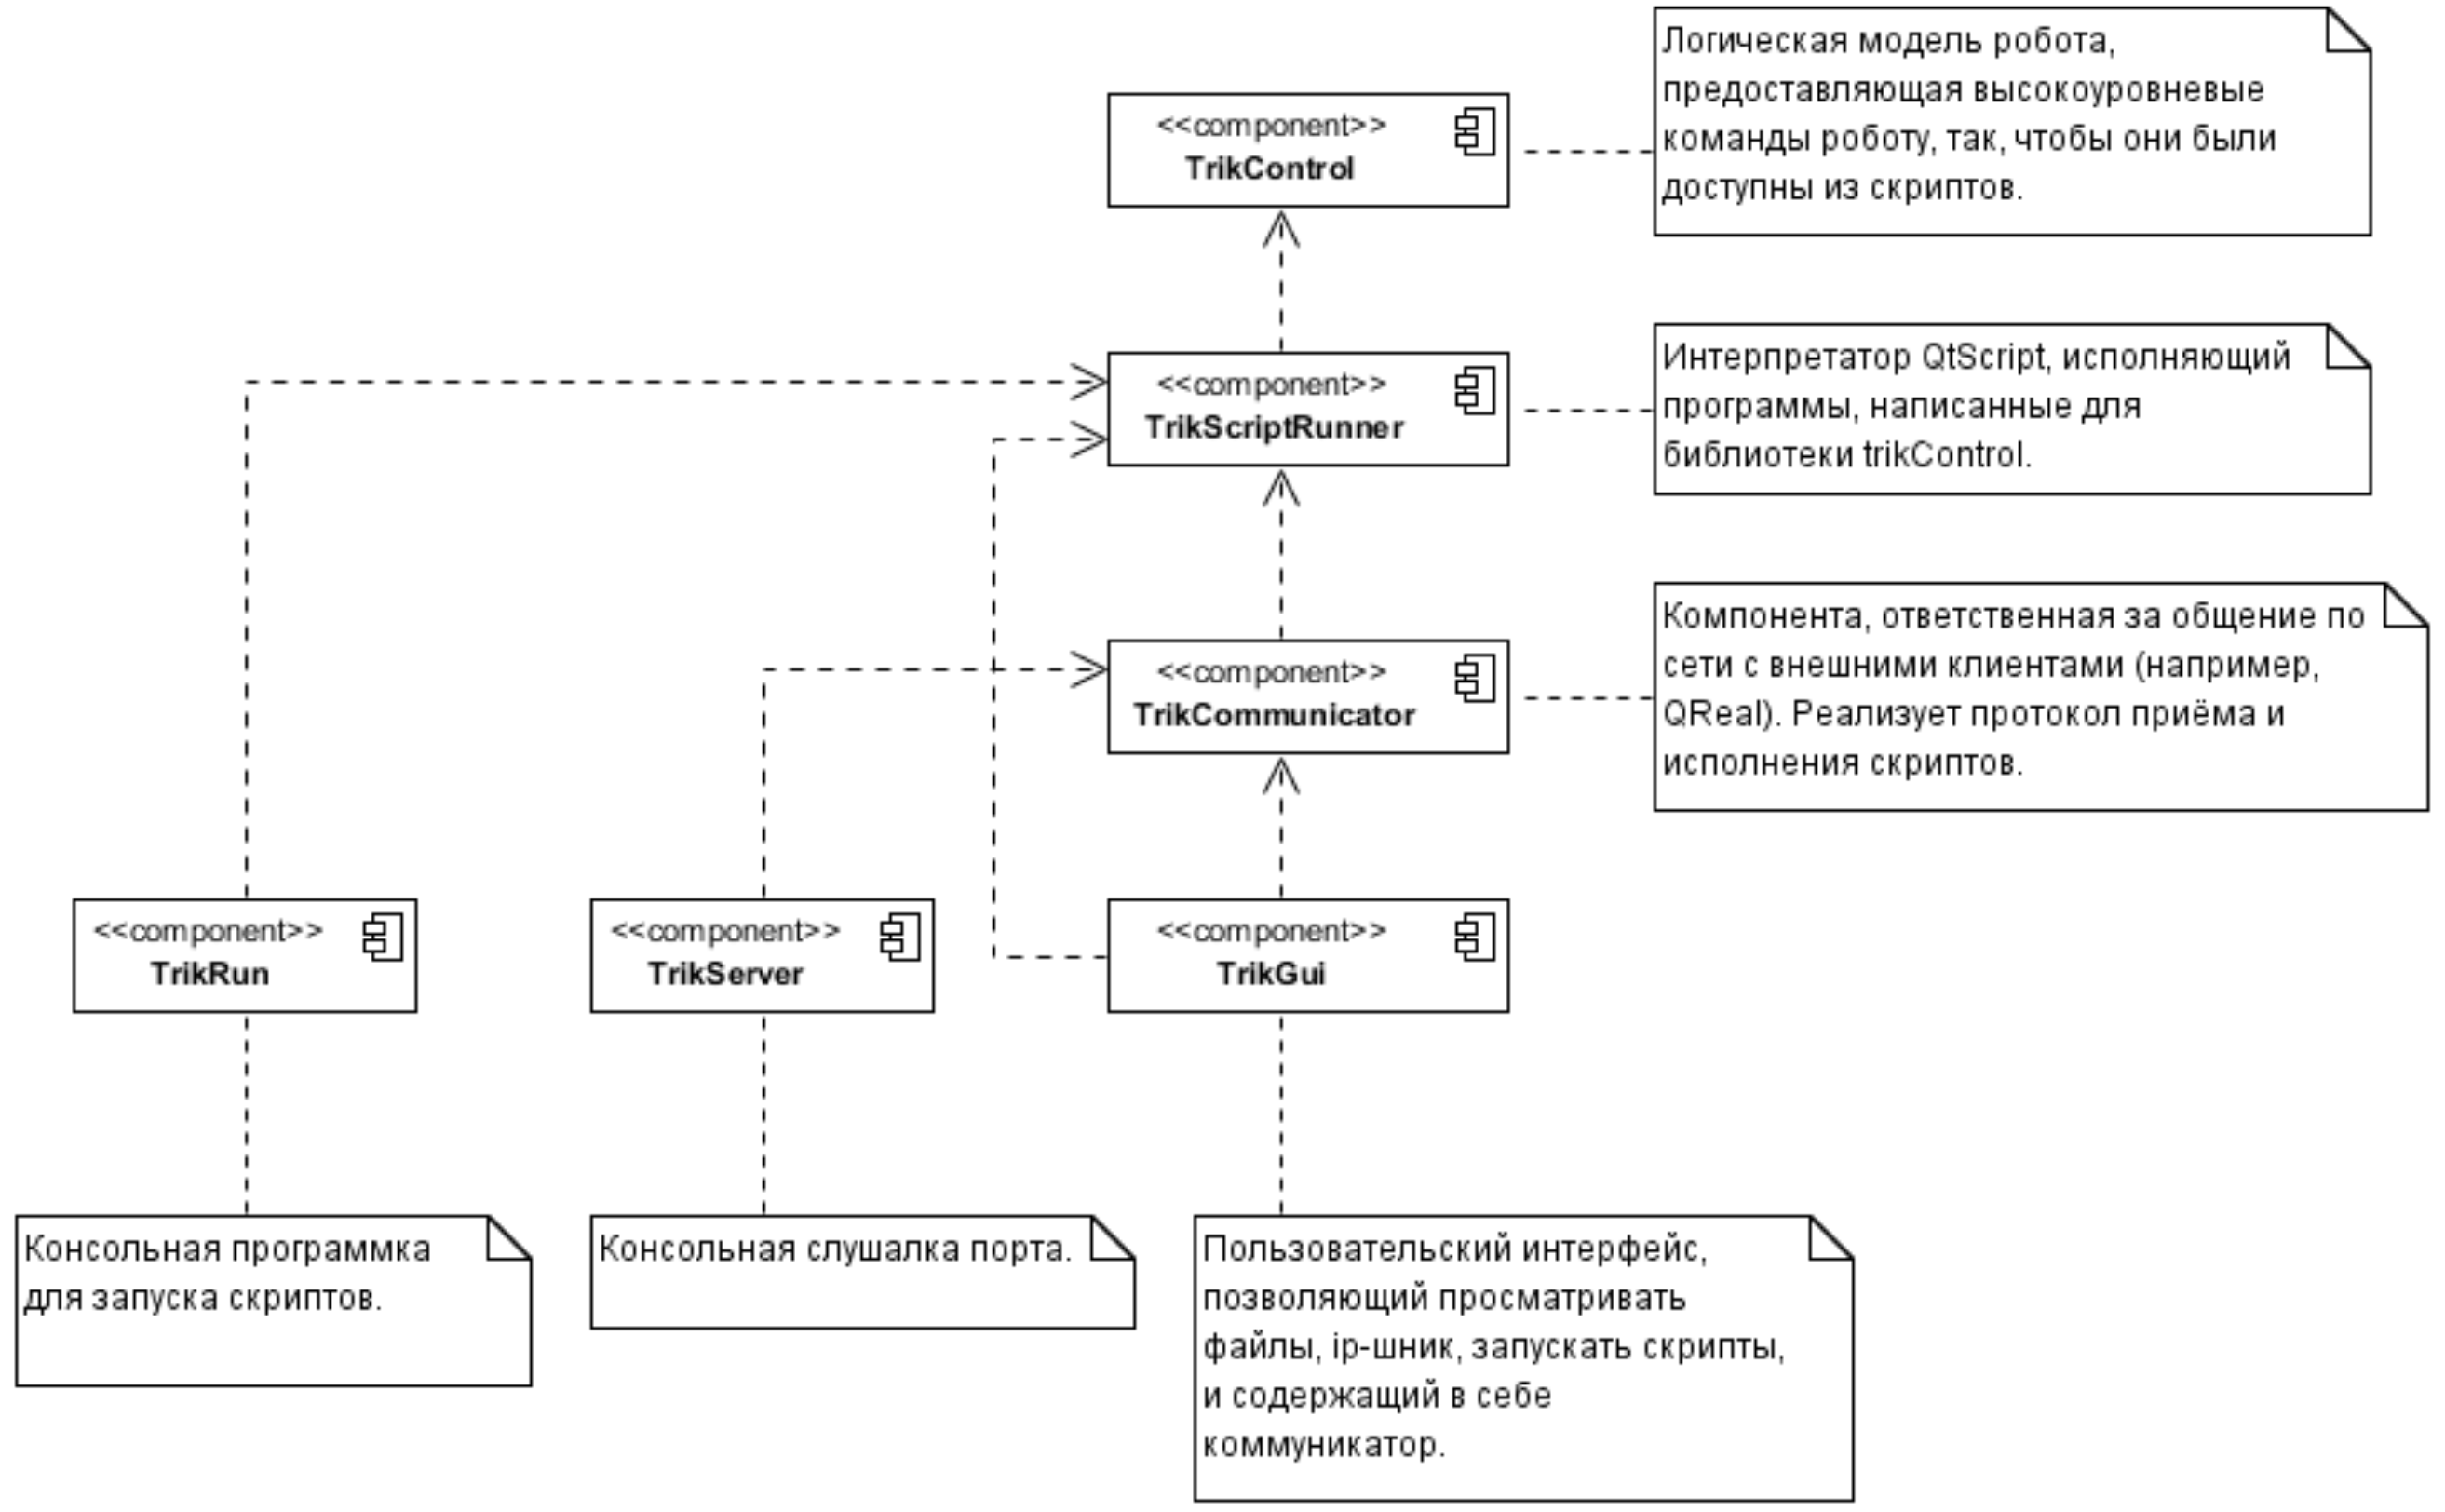
\includegraphics[width=0.9\textwidth]{componentDiagram.png}
        \end{center}
    \end{frame}

    \begin{frame}
        \frametitle{Ещё пример (UML)}
        \begin{center}
            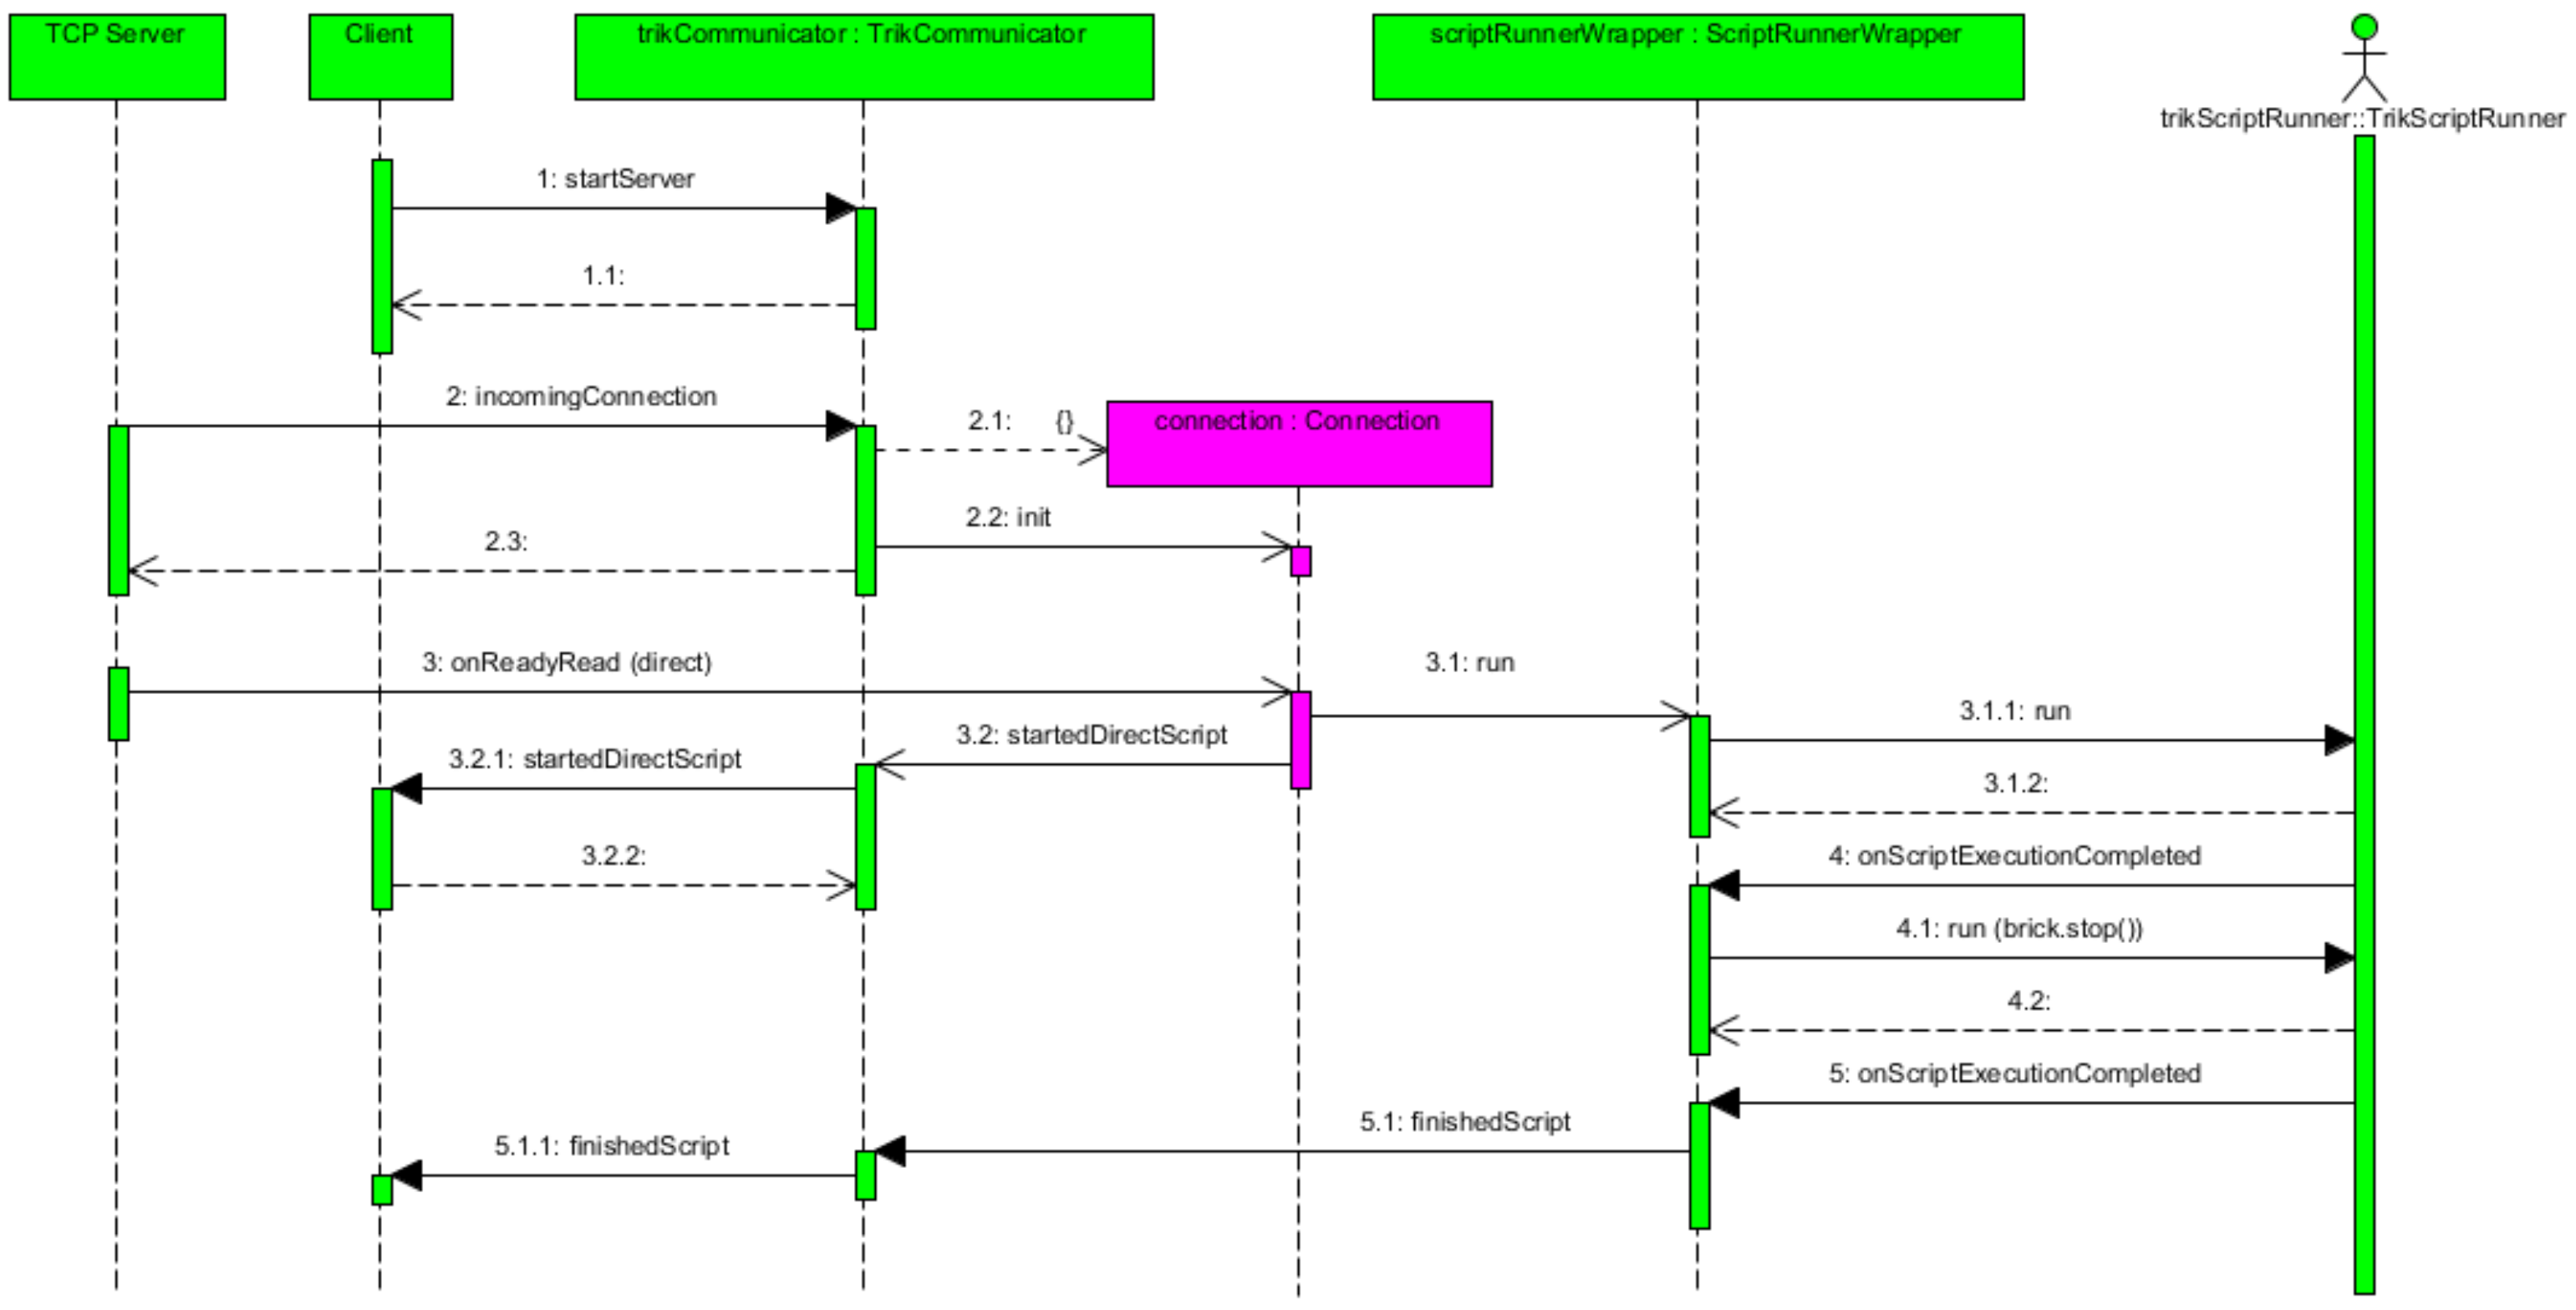
\includegraphics[width=\textwidth]{sequenceDiagram.png}
        \end{center}
    \end{frame}

    \begin{frame}
        \frametitle{UML, диаграммы классов}
        \begin{center}
            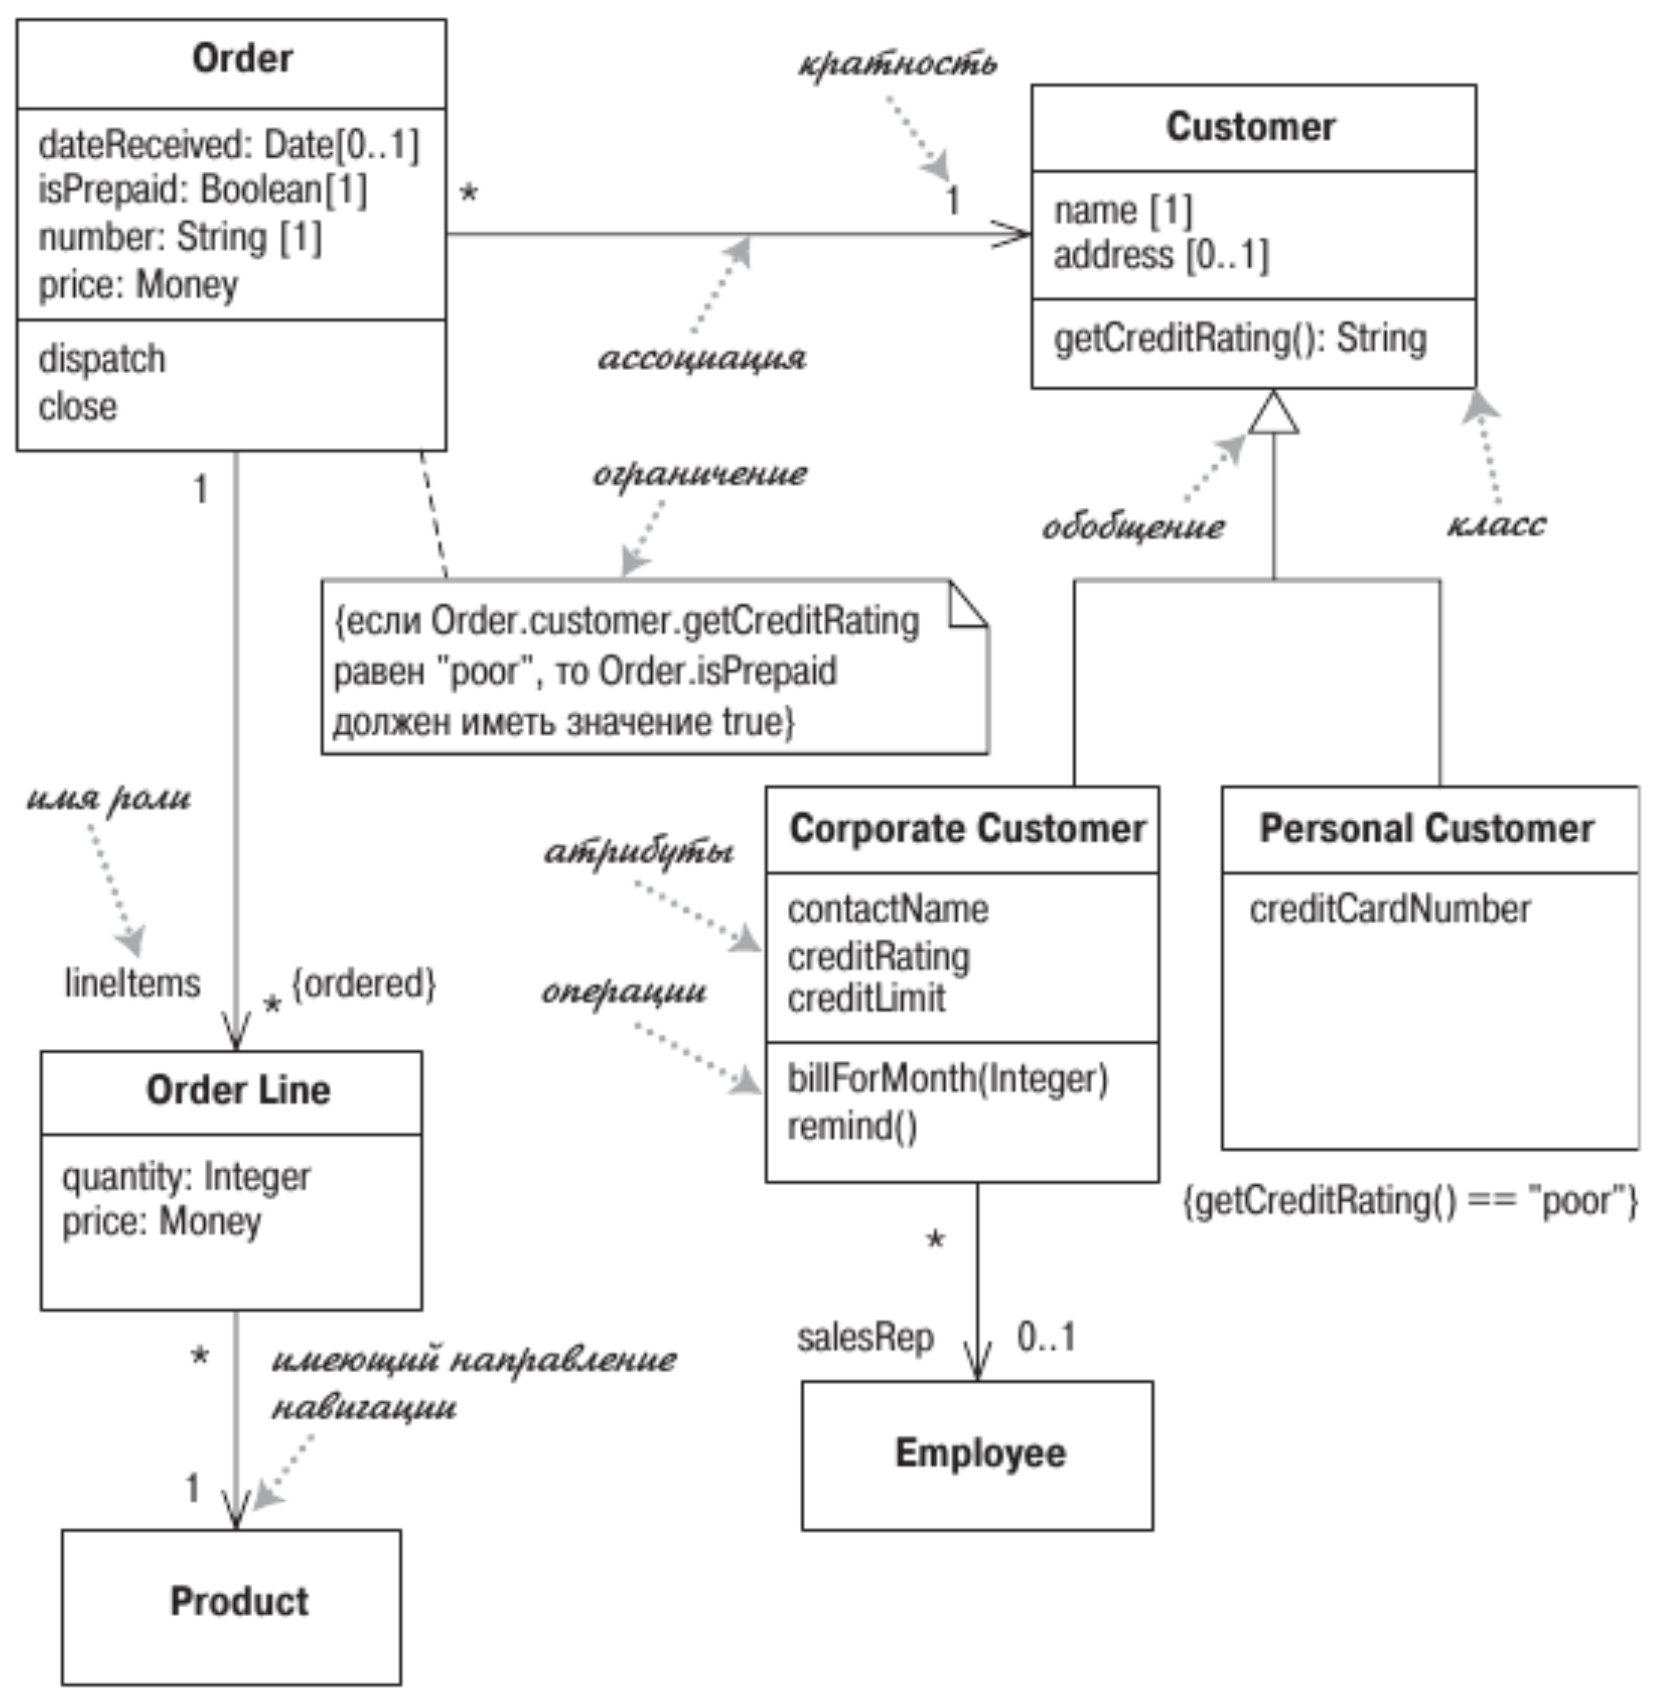
\includegraphics[width=0.6\textwidth]{classDiagram.png}
        \end{center}
    \end{frame}

    \begin{frame}
        \frametitle{Предметно-ориентированное моделирование}
        \begin{itemize}
            \item Специальные языки и инструменты для конкретной задачи или группы похожих задач
            \item Благодаря узости предметной области можно генерировать полностью работающую программу по диаграмме
            \begin{itemize}
                \item Зато оно работает только для этой предметной области
            \end{itemize}
            \item Могут программировать даже непрограммисты
        \end{itemize}
    \end{frame}

    \begin{frame}
        \frametitle{Пример: TRIK Studio}
        \begin{columns}
            \begin{column}{0.5\textwidth}
                \begin{itemize}
                    \item Среда программирования роботов
                    \item Программа --- набор элементарных команд
                    \begin{itemize}
                        \item Исполняются на реальном роботе по WiFi, Bluetooth, USB
                        \item Генерируются в код на текстовом языке и загружаются на робот
                        \item Исполняются на двумерной модели
                    \end{itemize}
                    \item Можно программировать только роботы
                    \item Могут программировать даже дети, не умеющие ещё читать
                \end{itemize}
            \end{column}
            \begin{column}{0.5\textwidth}
                \begin{center}
                    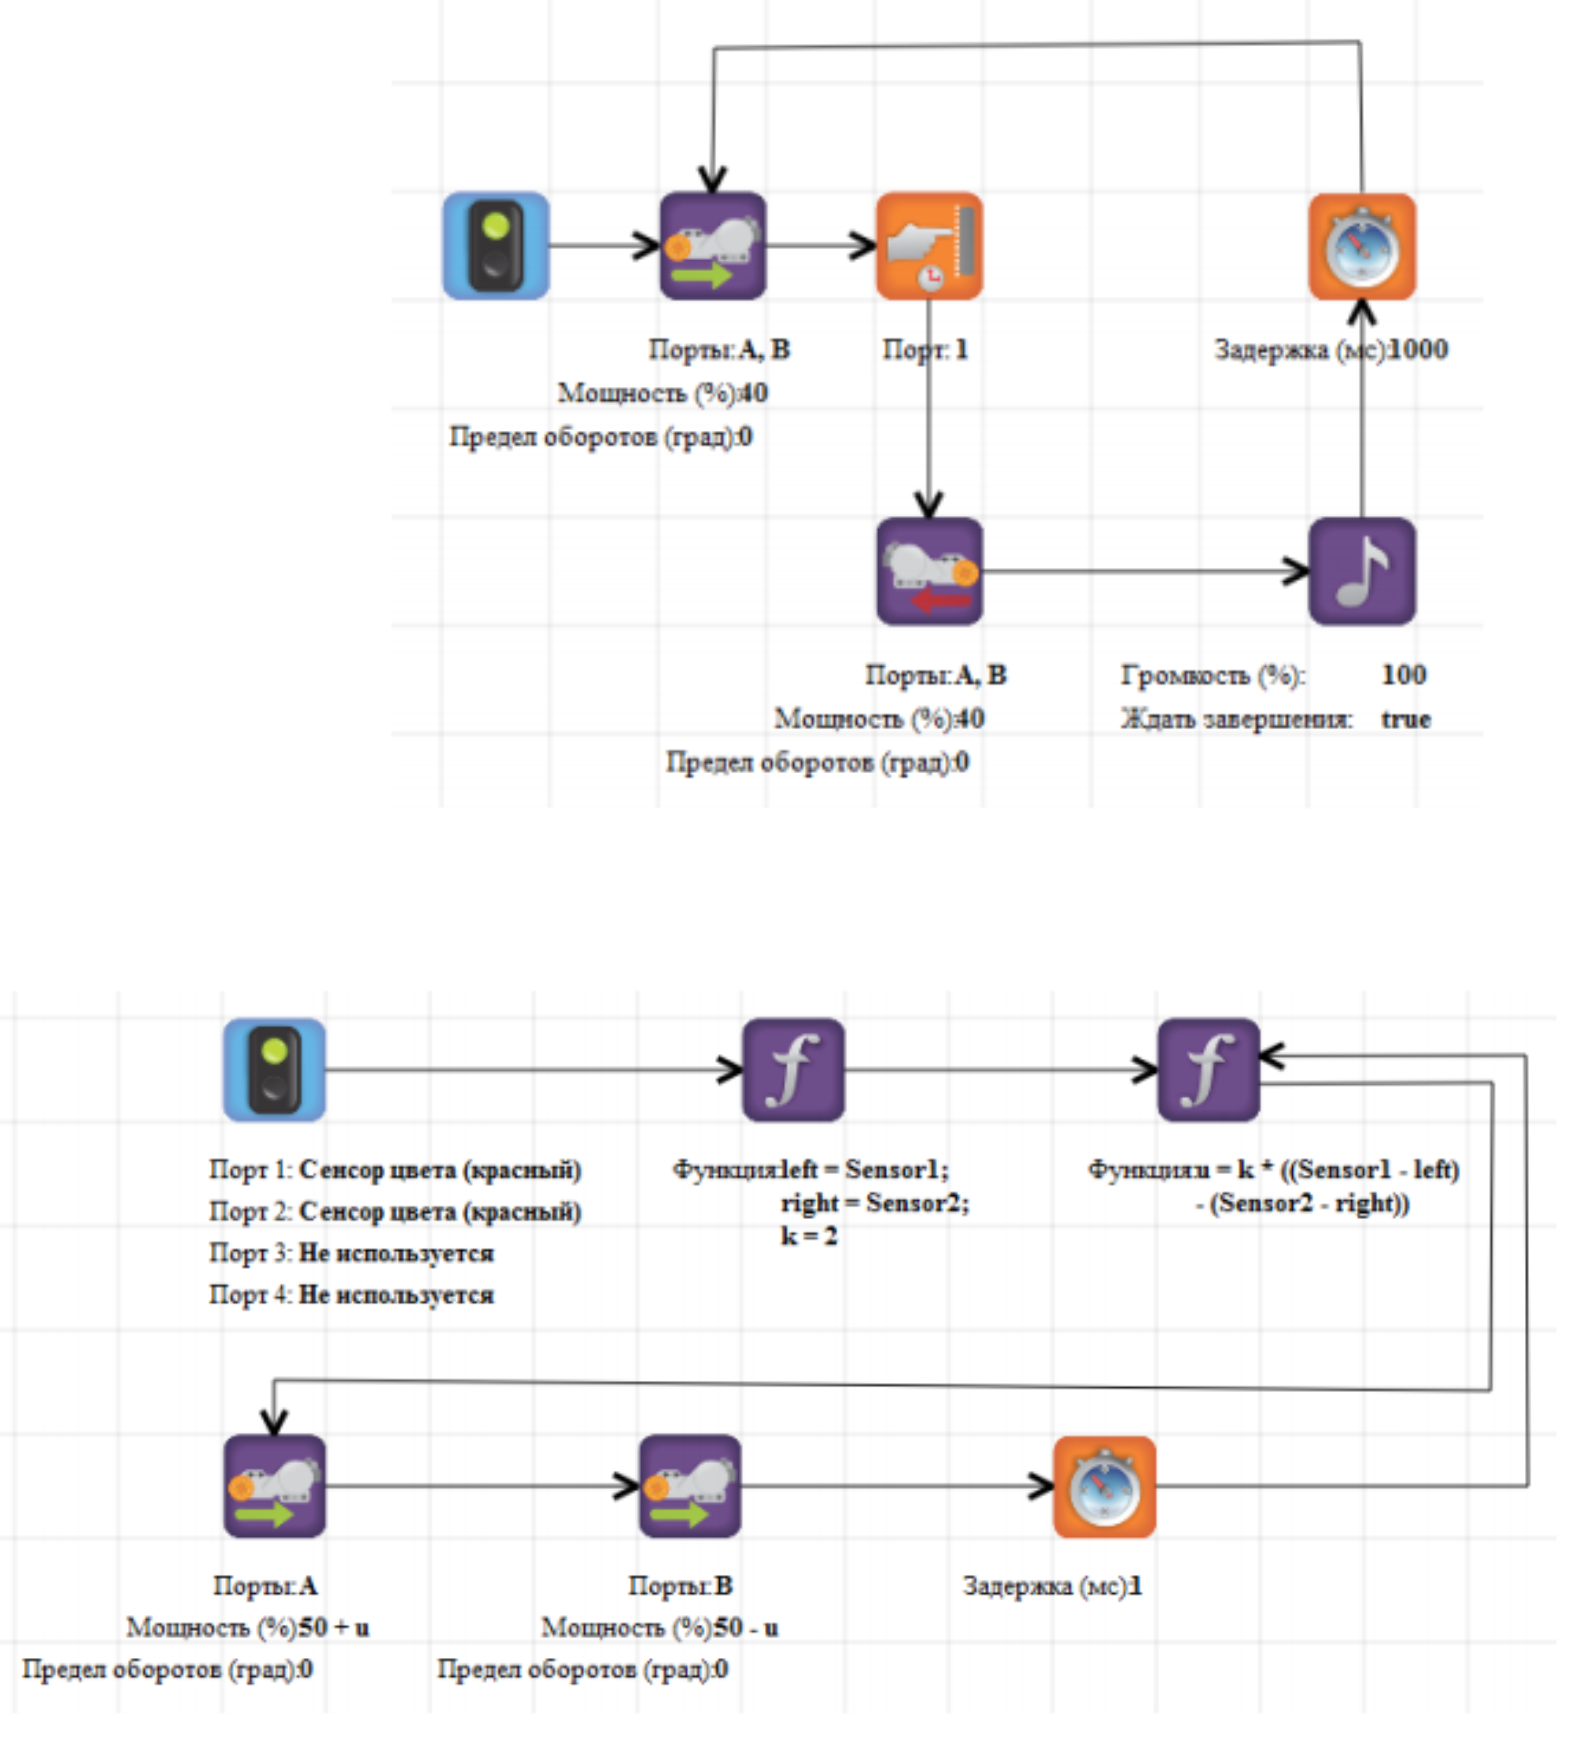
\includegraphics[width=\textwidth]{trikStudio.png}
                \end{center}
            \end{column}
        \end{columns}
    \end{frame}

\end{document}